\documentclass[aps,article,author-year,notitlepage,showpacs]{revtex4-1}
%\documentclass[a4paper]{article}

\usepackage{color}
\usepackage{graphicx}% Include figure files
\usepackage{enumerate}
\usepackage{amssymb,amsmath}
\usepackage{bm}% bold math
\usepackage{bbold}

\graphicspath{{./figures/}{./}}


\begin{document} 

\large

\noindent {\bf DG12856 Yin}\\

\noindent authors: Shi Yin, Rui Wen, and Wei-jie Fu\\

\noindent We are grateful to the referee for his comments and suggestions, which we have taken into account in the revised version:\\[0.3ex] 

The referee's comment on the influence of the splitting effect on thermodynamical observables are interesting, and we agree with it. So we modify the relevant statements in Sec. IV A and Sec. V.\\[0.3ex] 

\noindent \underline{A. Response to the physics questions}:\\

\begin{enumerate}[1.]

\item We follow the referee's suggestion, i.e., multiplying the longitudinal anomalous dimension $\eta_{\phi,k}^{\parallel}$ by a factor of 10, and increasing the splitting artificially. We have performed all the calculations with such artificial splitting and compare it with the real one in detail for several observables. The relevant results are presented in Fig. \ref{fig:z} through Fig. \ref{fig:kur} at the end of this response. We find that with the increase of the splitting of the meson wave function renormalization, its influence on the thermodynamical observables grows. In another word, this indicates that although $O(4)$ symmetry is partially lost in the vacuum in our setup due to the use of the $3d$ regulator, this defect is not too harmful for extracting the thermal effects resulting from the nontrivial dispersion relations of mesons. Certainly, an improved regulator will be helpful to clarify this issue eventually. We have added a paragraph, ``{\it In order to investigate whether the partial loss of the $O(4)$ symmetry in the vacuum, arising ...}'' , on page 8 in the revised version to address this issue. \\[0.3ex] 


\item We accept the referee's suggestion and investigate the splitting effect on the meson contribution to the pressure, i.e., $p_\phi$. The corresponding result is presented in Fig.4 in the revised version, and a related discussion is given on page 8, ``{\it In the left panel of Fig.4, we investigate the splitting effect of the meson wave function renormalization on the pressure at finite temperature and vanishing baryon chemical potential. Only ...}''.\\[0.3cm] 

\end{enumerate} 




\noindent \underline{B. Response to the questions concerning the text}:\\

\begin{enumerate}[1.]

\item {\it LPA$'$ needs to be defined explicitly. } \\
 
In fact, we have specified LPA$'$ in the old version. In the revised version, we reword it a bit, ``{\it where a momentum-independent $Z_{\phi,k}$ is included in LPA$'$ in comparison to LPA, ...}'' on page 2.\\[0.3ex] 

\item {\it Can the authors justify why $Z_{\sigma} = Z_{\pi}$, while their mass functions are very different?} \\

We have discussed this issue below Eq.(9). ``{\it The difference of the anomalous dimension between the $\pi$ and $\sigma$ mesons is neglected here. Note that even they are different, choosing the $\pi$-meson anomalous dimension for $\eta_\phi$, as done in this work, could minimize the errors of calculation, at least when the baryon chemical potential is not very high, since the mass of the pion is less than that of $\sigma$-meson, because of its nature of Goldstone particle, and the number of the degrees of freedom for the pions is also larger. Therefore, the mesonic degrees of freedom are dominated by the pions. But we should mention that, in the region of  high baryon chemical potential in the phase diagram, especially near the CEP, the $\sigma$-mode is the most relevant collective mode and the mass of the $\sigma$-meson is vanishing, it is necessary to distinguish the anomalous dimensions of $\pi$- and $\sigma$-mesons, which will be investigated in the future.}'' \\[0.3cm] 

\item {\it Fig.1: Please clarify whether all the Z's at UV point are the same, and what are the values?}\\

We have clarified this point in the text below Eq.(39) in the revised version, ``{\it Note that values of the wave function renormalizations at the UV cutoff are irrelevant for the computation, since only the anomalous dimensions, rather the wave function renormalizations themselves, enter into the flow equations.}'' \\[0.3cm] 

\item {\it Fig.1: Please comment on whether there are interesting differences at finite $\mu$.}\\

Similar results are also found for finite baryon chemical potentials, and we have commented on it in the caption of Fig.1 in the revised version.\\[0.3ex] 

\item {\it I assume the Polyakov loop value is obtained from a mean field calculation similar
to the study in Ref. Phys.Rev.C83:054904,2011. Please clarify.}\\

No, it is not a mean field calculation. The Polyakov loop is obtained self-consistently from their equations of motion, see, e.g., arXiv:1508.06504 for more details. We have addressed it below Eq.(12) in the revised version,  ``{\it where all the fields are on their respective equations of motion, see...}''.\\[0.3ex] 

\item {\it p.6 right column: spacial (or spatial?)}\\

We have modified it to ``spatial'', but we think both are okay.\\[0.3ex] 

\item {\it Fig.8: At low temperature, the Polyakov loop is more appropriately approximated as 0 rather than 1. Can the authors comment on what happens to the scheme dependence there?}\\

When the value of the Polyakov loop is set to be 1, the Polyakov-loop improved quark-meson model is reduced to be the usually used quark-meson model. So, we should not choose 0.\\[0.3cm] 

\end{enumerate}

Furthermore, we have corrected some typos in the manuscript and updated the references.\\[0.3cm] 


\noindent \underline{New figures response to question A1}:\\


%
%%%%%%%%%%%%%%%%%%%%%%%%%%%%%
\begin{figure}[htb]
\includegraphics[width=0.5\textwidth]{z}
\caption{Transversal and longitudinal wave function renormalizations for the mesons, $Z_{\phi,k}^{\perp}$, $Z_{\phi,k}^{\parallel}$, as functions of the RG scale $k$ in the vacuum obtained through increasing the longitudinal anomalous dimension $\eta_{\phi,k}^{\parallel}$ by a factor of 10 artificially (red and green lines), in comparison to the case without the artificial increase of the splitting (black and blue lines).}\label{fig:z}
\end{figure}
%%%%%%%%%%%%%%%%%%%%%%%%%%%%%
%

%
%%%%%%%%%%%%%%%%%%%%%%%%%%%%%
\begin{figure}[htb]
\includegraphics[width=0.5\textwidth]{m}
\caption{Meson masses as functions of the temperature at $\mu_B=0$, obtained through increasing the longitudinal anomalous dimension $\eta_{\phi,k}^{\parallel}$ by a factor of 10 artificially, in comparison to the case without the artificial increase of the splitting.}\label{fig:m}
\end{figure}
%%%%%%%%%%%%%%%%%%%%%%%%%%%%%
%

%
%%%%%%%%%%%%%%%%%%%%%%%%%%%%%
\begin{figure}[htb]
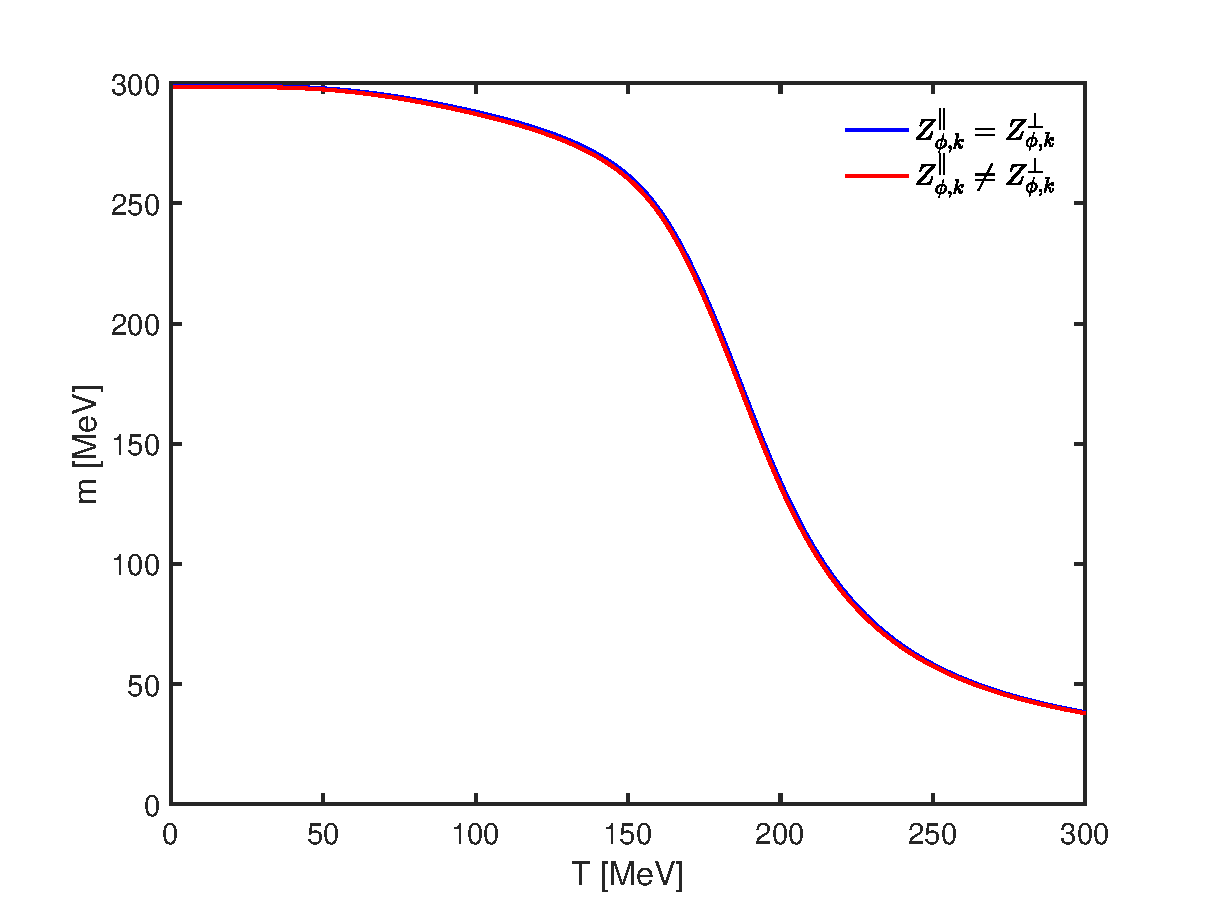
\includegraphics[width=0.5\textwidth]{mf}
\caption{Quark mass as a function of the temperature at $\mu_B=0$, obtained through increasing the longitudinal anomalous dimension $\eta_{\phi,k}^{\parallel}$ by a factor of 10 artificially, in comparison to the case without the artificial increase of the splitting.}\label{fig:mf}
\end{figure}
%%%%%%%%%%%%%%%%%%%%%%%%%%%%%
%

%
%%%%%%%%%%%%%%%%%%%%%%%%%%%%%
\begin{figure}[htb]
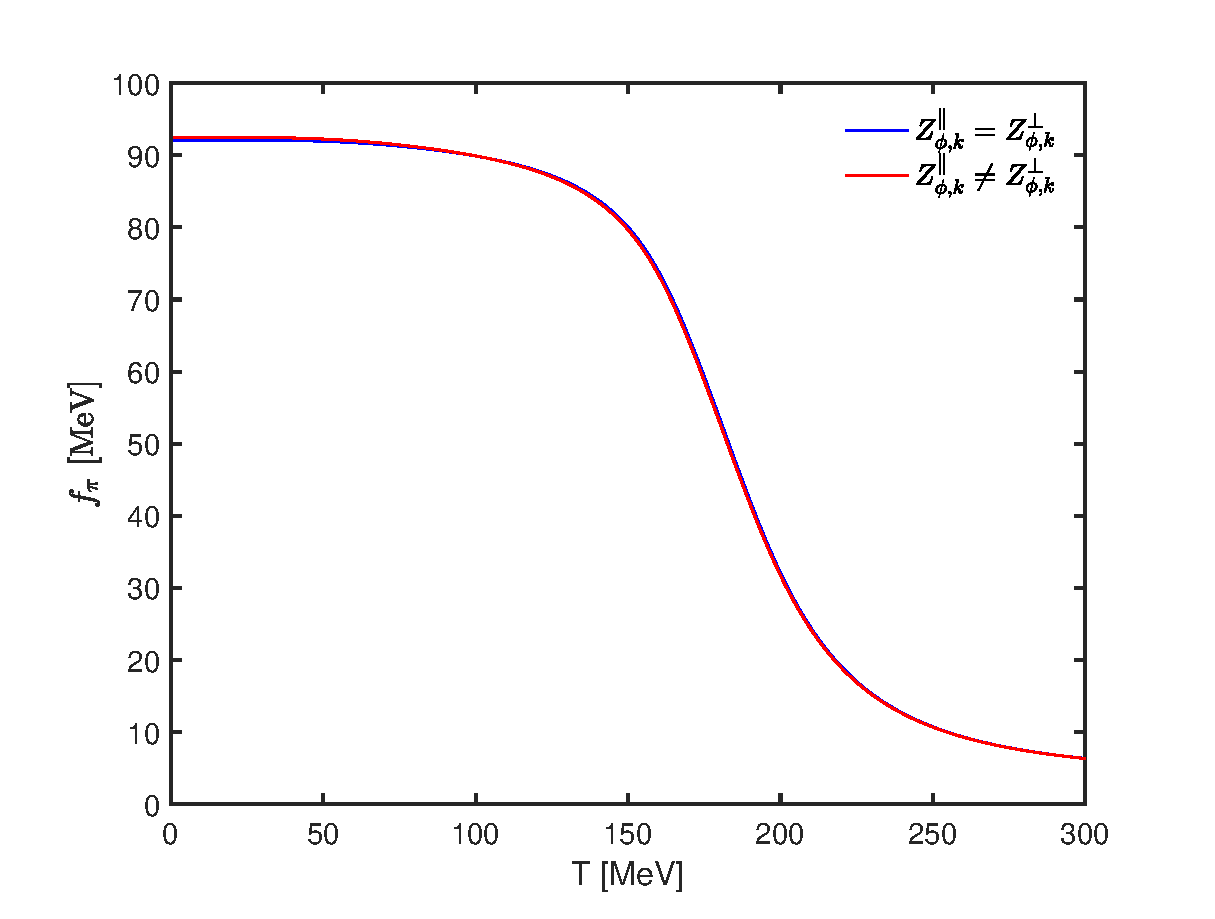
\includegraphics[width=0.5\textwidth]{fpi}
\caption{$f_\pi$ as a function of the temperature at $\mu_B=0$, obtained through increasing the longitudinal anomalous dimension $\eta_{\phi,k}^{\parallel}$ by a factor of 10 artificially, in comparison to the case without the artificial increase of the splitting.}\label{fig:fpi}
\end{figure}
%%%%%%%%%%%%%%%%%%%%%%%%%%%%%
%

%
%%%%%%%%%%%%%%%%%%%%%%%%%%%%%
\begin{figure}[htb]
\includegraphics[width=1.\textwidth]{chi}
\caption{Quadratic and quartic baryon number fluctuations $\chi_2^B$ (left panel) and $\chi_4^B$ (right panel) as functions of the temperature at $\mu_B=0$, obtained through increasing the longitudinal anomalous dimension $\eta_{\phi,k}^{\parallel}$ by a factor of 10 artificially, in comparison to the case without the artificial increase of the splitting.}\label{fig:chi}
\end{figure}
%%%%%%%%%%%%%%%%%%%%%%%%%%%%%
%

%
%%%%%%%%%%%%%%%%%%%%%%%%%%%%%
\begin{figure}[htb]
\includegraphics[width=0.5\textwidth]{kur}
\caption{Kurtosis of the baryon number distribution $\kappa \sigma^2=\chi_4^{B}/\chi_2^{B}$ as a function of the temperature at $\mu_B=0$, obtained through increasing the longitudinal anomalous dimension $\eta_{\phi,k}^{\parallel}$ by a factor of 10 artificially, in comparison to the case without the artificial increase of the splitting.}\label{fig:kur}
\end{figure}
%%%%%%%%%%%%%%%%%%%%%%%%%%%%%
%















\end{document}
